\documentclass{IOS-Book-Article}

\usepackage[super]{nth}
\usepackage{mathptmx}
\usepackage{hyperref}
\usepackage{tikz}
\usetikzlibrary{automata,arrows,positioning,calc}


\begin{document}
\begin{frontmatter}

\pretitle{Proposal}
\title{Markov Model To Estimate Expected Points For Volleyball Games With Limited Available Data}
\runningtitle{Limited-Data Volleyball Markov Model}
%\subtitle{Subtitle}

\author[A]{\fnms{Jack} \snm{Mooney}%
\thanks{Corresponding Author: Software Engineer and Proud Volleyball Parent}},
\author[A]{\fnms{Mark} \snm{Oglesby}}
and
\author[A]{\fnms{Rachael} \snm{Ritchie}}

\runningauthor{J. Mooney et al.}
\address[A]{Oconee County High School, Watkinsville, Georgia}

\begin{abstract}
Lorem ipsum.
\end{abstract}

\begin{keyword}
volleyball amateur high-school markov
\end{keyword}
\end{frontmatter}

\thispagestyle{empty}
\pagestyle{empty}

\section{Introduction}
Statistical analysis for volleyball at the high-school level is typically limited to the
collection of conventional statistics, e.g. kills, assists, aces, etc.  These stats, however,
fail to tell the whole story of which action and which player led to win or loss of a point. 
For example, consider a home-team outside hitter that makes an outstanding attack, which the 
visiting libero is barely able to dig into an overpass; this overpass results in a first-ball 
kill by the home middle.  Using conventional statistics, the middle is credited with a kill, and the outside is credited with a zero attack.  Who was actually more responsible for scoring the point?

Clearly the middle would not have had such an easy kill without the outside's attack.  And 
perhaps the hitter would not have been able to take the attack angle she had without the
setter putting the ball in exactly the right place; and the setter may not have been able to 
make that set without a good pass from the back row; and such a pass may have been only 
possible because the visiting team had to return the previous attack as a freeball ... and so 
on. Thus the chain of events that resulted in a point continues all the way back to the serve.

The solution for estimating the contribution of different players to a team goal is to
estimate the effect of any individual action on likelihood of scoring (and necessarily being 
scored upon). The chained-event nature of volleyball lends itself well be being modeled by a 
Markov chain.

Markov models have been used many times to model the scoring probabilities of various 
situations in volleyball. \cite{xu, flo, aldous} One common theme of all of the referenced studies 
is that the data comes from DataVolley- or Volleymetrics-based annotation of NCAA and international competition.

High school volleyball, on the contrary, presents a challenge for modeling:
\begin{enumerate}
    \item Touch-by-touch data does not exist in any significant quantity (in contrast to NCAA, pro,
    and Olympic levels).
    \item In fact, any data at all tends to be scarce because of the limited amount of video 
    available to any one coach or scout, and the fact that all data collection is done by volunteers
    or school teachers for whom coaching is an additional duty.
    \item There is so much variation in team quality that many match-ups are quite lopsided, meaning
    that certain events that are unlikely in high level competition (such as a ``freeball kill'') 
    are over-represented. 
\end{enumerate}

This paper presents a simplified Markov model for volleyball rallies which can be fed with a comparatively small amount of rally data to identify the transition matrix.

\section{General Approach}

\subsection{Definitions}

\begin{description}
\item [Match] A sequence of ``best of 3'' or ``best of 5'' sets.
\item [Set] A sequence of rallies. Set winner is the first team to score 25 points and exceed the
opponent's point total by 2 or more. For the final (\nth{3} or \nth{5}) set in a match, 15 points
is the goal.
\item [Run] A sequence of rallies where one team serves consecutively.
\item [Rally] A sequence of events which begins with one team serving, and ends with either team
scoring a point.
\item [Possession] A sequence of consecutive touches by a single team; by rule no more than 4
touches including an attempted block.
\item [Touch] Any time any player touches the ball.
\end{description}

\subsection{Markov Model States}

Data is gathered from the Georgia High School Association 2022 AAA volleyball state tournament to 
ensure that the match-ups are relatively even, and that the level of play is high enough to avoid 
having randomness dominate the results.  Additionally, this is dataset readily available to the 
authors, one of the goals of this research is to find an expected point model using the data
available to a typical high-school coaching staff.

The key driver of point outcomes in volleyball, aside from errors, is the touch location, ball 
trajectory (high, medium, low), and destination and  of each touch; however, the size of possible 
states is large. Consider that a touch could happen in 6 possible court locations, have 3 
categories of trajectories, and 12 possible court locations as destinations; there are 216 
possible states. That number only increases if more detail is added.  In the available dataset, 
there are, at best, 65,000 \footnote{31 matches, 210 points if every match is 3-2, and every set 
is 25-23 or 15-13, assume average 10 touches per point} touches. Note, however, that the vast 
majority of those touches will be bucketed into a few common categories--serve to back row, high 
set from middle front court to left front court, etc.--such that transitions to and from certain 
states will be poorly represented.

In the interest of keeping the space of possible states/events in the model small, but still 
representative, we propose a model that does not register individual touches, but instead the
combined outcome of a team's possession.  These outcomes are

\begin{description}
    \item [Serve (s)] A serve by the conventional definition. This is a starting state that is never
          returned to.
    \item [Deliberate Attack (d)] Any above-the-net attack in which the setter plays the ball near
          center-front court without having to run to the ball, and has the ability to set to 2 or 
          more attackers. An exception to the above-the-net rule is a setter dump.
    \item [Improvised Attack (i)] Any above-the-net attack which does not meet the above criteria.
    \item [Continue Rally Play (c)] A touch that sends the ball over the net on the \nth{2} or 
          \nth{3} touch of the possession, with the intent of merely continuing the rally without
          intent of immediately scoring a point.
    \item [Block (b)] An above-the-net \nth{1} touch to defend against an a attack where the ball
          immediately bounces back into the attacker's side of the court.
    \item [Overpass (o)] A \nth{1} touch that arcs back over the net; often the result of a dig or         pass that is contacted just a bit too hard.
    \item [First Touch Attack (1)] A \nth{1} touch where the attacker is attempting to immediately
          score a point (often in response to an overpass).
    \item [Point Scored (p)] When the last team to take one of the above actions scores a point
          (conventionally recorded as an ace, kill, or block) Terminal state.
    \item [Point Relinquished (e)] When the last team to take one of the above actions gives up 
          a point (conventionally recorded as an error). Terminal state.
\end{description}

Note that these definitions try to avoid using some conventional volleyball terminology such as 
in-system or out-of-system attack or freeball.  This is to avoid baggage of pre-existing notions
of, for example, what is in-system or out.  Under these definitions, a team could be in-system but
because of a timing mistake ends up missing a swing--that would be a defensive shot. Additionally,
``block'' as defined above includes block kills, block errors, and covered blocks, but not block
attempts that are played by the blocker's teammates. Downballs and freeballs, while distinct, often
have the same intent and effectiveness--continue the rally.

\subsection{Expected Point Value}

The long term probabilities of scoring from any state are inferred using eigenvector analysis of the
Markov transition matrix \cite{mit}. That probability of scoring is converted into an expected point
value for each state \cite{gordonprobwin}.

The changes in expected point value from state-to-state can be attributed to specific players on 
each transition.  These expected point transitions are zero-sum; i.e. expected point value gained by
a hitter's attack is lost by any players that attempt to block and/or dig. For certain situations, 
for example an error on a double hit or net violation, the gained point value is distributed to the 
entire opposing team. Annotating this data has the added benefit of clearly noting the player 
match-ups inherent in each event.

In this way the sum total of all expected points added for every player on the team, less the number
of times they served times the expected value at serve, should equal the point differential between
the two teams at the end of a set.

This attribution allows coaches to much more clearly see each player's contributions toward winning 
or losing.  Additionally, the total expected points added, the expected points added per rally, and 
the expected points added per touch should be quite informative.

\subsection{Caveats}

Because our own team is will be strongly over-represented in the data available to us, we have two
choices. First, we can develop the model presuming that the model is most accurate for our team or 
that our team is sufficiently representative of other teams in our class.  Alternatively, we can 
attempt to weight observations such that each team is as evenly represented as possible.

The authors acknowledge that this is a very reductive approach, but still has enough distinct
features to be able to glean insights about the game that may not be possible with a more granular
approach due to randomness from the lack of data.

Questions for other authors in this proposal:
1. Are these the right states? We could, for example, split 'Defensive Shot' into downball and 
freeball, if the results of these events are different enough.
1.5. How to record tools? p-b-e or p-s
2. Do we need to include serve receive versions of these states as distinct?
3. How to handle net errors and ball handling errors? (Try to classify what would have happened and 
then record it as pr.  E.g. a perfect pass but the setter double-hits would be p-d-e.  A net error on
attempted block would be p-b-e.
4. Other authors? A math teacher?

\subsection{Theoretical Model / Markov States}
\begin {figure}
\centering
	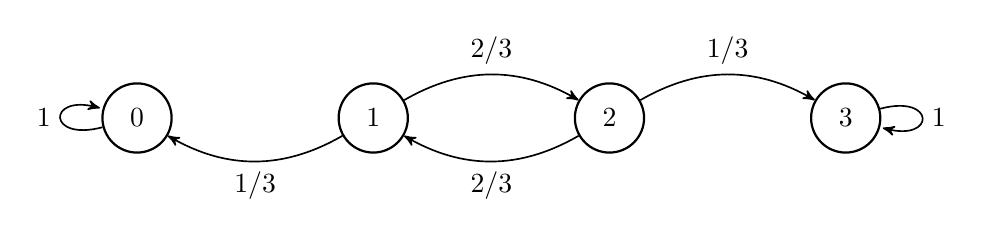
\begin{tikzpicture}[->, >=stealth', auto, semithick, node distance=3cm]
	\tikzstyle{every state}=[fill=white,draw=black,thick,text=black,scale=1]
	\node[state]    (A)                     {$0$};
	\node[state]    (B)[right of=A]   {$1$};
	\node[state]    (C)[right of=B]   {$2$};
	\node[state]    (D)[right of=C]   {$3$};
	\path
	(A) edge[loop left]			node{$1$}	(A)
	(B) edge[bend left,below]	node{$1/3$}	(A)
	edge[bend left,above]		node{$2/3$}	(C)
	(C) edge[bend left,below]	node{$2/3$}	(B)
	edge[bend left,above]		node{$1/3$}	(D)
	(D) edge[loop right]		node{$1$}	(D);
	%\node[above=0.5cm] (A){Patch G};
	%\draw[red] ($(D)+(-1.5,0)$) ellipse (2cm and 3.5cm)node[yshift=3cm]{Patch H};
	\end{tikzpicture}
\caption{Markov model}
\label{fig:markov_model}
\end{figure}

\subsection{Data Gathering}

Here I want notes about how each match is to be annotated.

s,p,i,p,p,b,i,d,d,ps (Kill from a planned attack)

s,pr (Service Error)

s,ps (Service Ace)

s,d,i,d,d,b,pr (Block error)

s,d,i,d,d,b,ps (Block kill)

\subsection{Model Training and Validation}

The model will be validated by randomly assigning event pairs into an A group and B group and train 
the model with each group. The expected point value for each state/event should differ by no more 
than 5\%.

\section{Applications}

\subsection{Player performance evaluation}

* Own players -- who should start, when to sub
* Opposing players -- who to "pick on" with service and hits

\subsection{Practice time allocation}

Which aspects of the game have the most potential to increase scoring.

\subsection{Serve aggressiveness}

How many aces are worth absorbing an error?

\begin{thebibliography}{99}

\bibitem{xu}
Xu, Brian, \textit{A Markov Model for Volleyball}. Department of Statistics, Rice University, \url{https://bzx24.github.io/static/media/paper.1f751159.pdf} August 2021.

\bibitem{flo}
Florence, Lindsay W. Fellingham, Gilbert W. Vehrs, Pat R. and Mortensen, Nina P. (28) ``Skill
Evaluation in Women's Volleyball,'' \textit{Journal of Quantitative Analysis in Sports}: Vol. 4:Iss.
2, Article 14. Accessed at 
\url{https://scholarsarchive.byu.edu/cgi/viewcontent.cgi?article=1192&context=facpub}.

\bibitem{aldous}
Aldous, David J. and Cruz, Madelyn, ``A Real-World Markov Chain arising in Recreational Volleyball'', \textit{Involve: a journal of mathematics}, 2021.

\bibitem{trinsey}
Trinsey, Joe. ``The Triangle.'' Smarter Volley, 1 November 2021, 
\url{https://smartervolley.substack.com/p/thetriangle}.

\bibitem{gordonev}
Gordon, Chad. ``Step 10: Expected Value Added (eV+) For All Skills.'' Rethinking Volley, 15 August 
2020, 
\url{https://volleydork.blog/2020/08/15/step-10-expected-value-added-ev-for-all-skills/}.

\bibitem{gordonprobwin}
Gordon, Chad. ``Step 11.5: Probability to Win the Point, Expected Value, and Other Metrics. A Quick Pitstop.'' Rethinking Volley, 2 September
2020, 
\url{https://volleydork.blog/2020/09/02/step-11-5-probability-to-win-the-rally-expected-value-and-other-metrics-a-quick-pitstop/}

\bibitem{mit}
``Lecture 8: Markov eigenvalues and eigenvectors'' \textit{MIT Opencourseware 6.262: Discrete 
Stochastic Processes} 28 February 2011
\url{https://ocw.mit.edu/courses/6-262-discrete-stochastic-processes-spring-2011/4c926d96cd76ee6427d207d0cc08b841_MIT6_262S11_lec08.pdf}.

\end{thebibliography}
\end{document}